\setcounter{page}{1}
\setcounter{figure}{0}  % reset counter


\section{Supplemental methods}
%As a first step to our method, given the dominant peptide identification $p$ from MS$^2$, the precursor mass $M$ from MS$^1$, and the set of modifications $Mods$, we enumerate all modification variants of $p$ that satisfy the precursor ion mass $M$. This can be done for each MS/MS spectrum by simple combinatorial enumeration of variants in exponential running time in the number of modifications. We propose a novel efficient algorithm to solve this problem.
%
%\old{
%Consider the tandem mass spectrum of peptide 'ARKTRAK' modified by about $42$ Da and $4$ types of modifications $\{$acetylation(Ac), methylation(Me), dimethylation(2Me) and trimethylation(3Me)$\}$. Due to the isobaric nature of 3Me and Ac (42.0470 and 42.0106 Da, respectively), the shift in the mass of the peptide can be explained by an Ac or a 3Me. The peptide has two potential sites for a Ac (Lysine(K);K3 and K7) and two potential sites for each of other modifications (Arginine(R); R2 and R5). Since modifications can occur in different combinations and at
%different sites, as shown in Figure~\ref{fig:illustration}, there are potentially $6$ distinct isobaric modification variants of this peptide that might lead to the MS/MS spectrum with the shifted precursor mass.
%\begin{figure}[htbp]
%\centering
%\includegraphics[width=0.8\textwidth]{figures/PTMQ_Example.pdf}
%\caption{Mixture MS/MS spectrum of isobaric peptide modification forms.}
%\label{fig:illustration}
%\end{figure}
%}
%
%We consider a peptide $p=a_1 a_2 \ldots a_L$ of length $L$, and a set of modifications $Mods=\{x_j=(a_{i_j},m_j)\}$, each defined by its amino acid specificity $a$, and induced non-zero mass offset $m\in \mathbb{R}$. Let $mass(p)=mass(a_1,a_2,\ldots,a_L)$ be the total mass of peptide $p$, defined as $\sum_{i=1..L} mass(a_i)$ for unmodified peptides. Using $a_i^{m_i}$ to indicate a modification of mass $m_i$ on the $i$-th amino acid, the mass
%of a modified peptide $p$ is defined as $\sum_{i=1..n} mass(a_i)+m_i$ where $m_i=0$ for unmodified amino acids.
%
%Given a peptide $p$, set of modifications $Mods$, and precursor mass $M\in \mathbb{R}$, the problem of modification variant enumeration is to list all modified peptide sequences $\Pi(p,Mods,M)=\{\pi^1,\pi^2,\ldots,\pi^{n_{\pi}}\}$ such that
%\begin{itemize}
%\item $\pi_i$ can be derived from $p$ by modifying amino acids with modifications in $Mods$,
%\item $mass(\pi_i)$ is $\in [M-t, M+t]$ for a mass tolerance $t\in \mathbb{R}$, and
%\item the number of modifications per amino-acid $a_i$ is at most $1$.
%\end{itemize}
%Each of these modified peptide sequences is referred to as a {\em modification variant} of $p$.
%
%This problem is a more generalized version of Subset-Sum Problem which is known as an NP-Complete Problem. In this problem, the items are the possible modifications in $Mods$ with values $m_j$ that correspond to modification masses and the target sum to be achieved is the difference between the precursor mass $M$ and the mass of the unmodified peptide $p$. However, the modification masses are not limited to positive integers, they can be non-integers and negative as well. Also, we need to consider the error in the estimation of the precursor mass $M$ by allowing the target sum to be within range $[\Delta M-t, \Delta M+t]$ where $\Delta M = M-mass(p)$.
%
%In the worst case, $|\Pi(p,Mods,M)| = 2^{|Mods|}$ and a naive exponential-time recursive solution that goes through all subsets of $Mods$ will enumerate all the variants that satisfy the given precursor mass in $O( 2^{|Mods|})$ time. However, in practice the number of variants that satisfy the precursor mass $M$ is much less than $2^{|Mods|}$. We propose the pseudo-polynomial time DP algorithm, shown in Figure~\ref{alg:ModVarEnum}, where the subproblems are defined on the subsets of $Mods$ and target values smaller than $\Delta M$. In the algorithm, before starting to solve subproblems, we first scale up the problem with a factor $f$ so that the modification masses $m_j$, mass difference $M$ and tolerance $t$ are all integers. The running time of this algorithm is $O((M+t)\cdot f\cdot |Mods|\cdot n_{\pi})$ where $n_{\pi}= |\Pi(p,Mods,M)|$ is the size of the solution.
%
%\begin{figure}[htb]
%\begin{algorithm}{Enumerate-Modification-Variants}
%\textbf{Input:} \text{ peptide} p, \text{Mods}=\{x_1, \cdots, x_n\}, \text{precursor mass } M,\quad \\
%\text{mass tolerance $t$, scaling factor $f$} \quad \\
%\textbf{Output:} \text{ all $S\subset$ Mods s.t. mass$(p)+\sum_{x_k\in S} m_k \in [M-t, M+t]$} \quad \\
%\Delta M\= M-mass(p) \\
%\Delta M\= \lfloor\Delta M\cdot f\rfloor \\
%t\= \lfloor t\cdot f\rfloor \\
%\begin{FOR} {j = 1 \text{ to } n}
%m_j\= \lfloor m_j\cdot f\rfloor
%\end{FOR}\\
%\text{Let A be an array of size $\Delta M+t+1$} \\
%\text{$A[m_1]\= \{\{x_1\}\}$, $A[i]\= \emptyset$ for all $i\neq m_1$} \\
%\begin{FOR} {\text{$j = 2$ to $n$}}
%    \begin{FOR} {\text{$i = \Delta M+t$ down to $m_j$}}
%        \begin{FOR} {S\in  A[i-m_j]}
%            \text{$A[i]\= A[i]\cup \{S\cup \{x_j\}\}$}
%        \end{FOR}
%    \end{FOR}
%\end{FOR}\\
%\RETURN \bigcup_{i=(\Delta M-t):(\Delta M+t)} {A_i}
%\end{algorithm}
%\label{alg:ModVarEnum}
%\caption{Pseudo-polynomial dynamic programming algorithm to enumerate all modification variants.}
%\end{figure}

%\begin{algorithm}
%\caption{Enumerate-Modification-Variants}
%\label{alg:VariantEnumDP}
%\begin{algorithmic}
%\STATE \textbf{input } peptide $p$, $Mods=\{x_1, \cdots, x_n\}$, precursor mass $M$, mass tolerance $t$, scaling factor $f$
%\STATE \textbf{output} all $S\subset Mods$ s.t.  $mass(p)+\sum_{x_k\in S} m_k \in [M-t, M+t]$
%\STATE $\Delta M\gets M-mass(p)$,
%\STATE $\Delta M\gets \lfloor\Delta M\cdot f\rfloor$
%\STATE $t\gets \lfloor t\cdot f\rfloor$
%\FOR {$j = 1$ to n}
%    \STATE $m_j\gets \lfloor m_j\cdot f\rfloor$
%\ENDFOR
%\STATE Let A be an array of size $\Delta M+t+1$
%\STATE $A[m_1]\gets \{\{x_1\}\}$, $A[i]\gets \emptyset$ for all $i\neq m_1$
%\FOR {$j = 2$ to $n$}
%    \FOR {$i = \Delta M+t$ down to $m_j$}
%        \FOR {$S\in  A[i-m_j]$}
%            \STATE $A[i]\gets A[i]\cup \{S\cup \{x_j\}\}$
%        \ENDFOR
%    \ENDFOR
%\ENDFOR
%\RETURN $\bigcup_{i=(\Delta M-t):(\Delta M+t)} {A_i}$
%\end{algorithmic}
%\end{algorithm}
%
%Note that the algorithm given in Figure~\ref{alg:ModVarEnum}  works for positive modification masses. It can be easily generalized for also negative values by solving the subproblems for the target values from $T^-$ to $T^+$ where $T^-$ is the sum of negative modification masses and $T^+$ is the sum of positive modification masses. Then, the running time becomes $O((T^+-T^-)\cdot f\cdot |Mods|\cdot n_{\pi})$ which is still polynomial in the number of modifications and the size of the solution.

\subsection{Inference of Fragment Ion Detectabilities}\label{sec:inferDetectabilities}
The idea behind our approach is that the observed intensity of a peak is
directly related to the total abundance of the theoretical fragment
ions that have the same corresponding m/z value, thus to the total
abundance of the modification variants that contain those isobaric
ions. Simply, if there is a peak in the spectrum which is associated
with a single modification variant through a single ion, the peak
intensity is a direct measurement for the abundance of the
modification variant. However, the fragment ions have different
intensities in the mass spectrometry depending on the
physico-chemical properties of the fragment ions. For our purposes,
only the relative contributions of the fragment ions to the peak
intensities per unit abundance of its parent peptide are
important.

For inference of expected ion intensities, we are motivated by
conservation of spectral shapes of a peptide sequence across different
unmodified and modified tandem mass spectra. Previously, Sniatynski et
al~\cite{Sniatynski2006}. showed that delay-series
correlation between the mass spectra of modified and unmodified
peptides revealed significant spectral overlap at an offset indicative
of the modification. This observation has been confirmed in many other
publications including ours~\cite{bandeira10chapter}. We
observe similar behavior in also our test MS/MS datasets.

We measure the similarity between two spectra using \emph{cosine score} which is a widely accepted measure for
spectral similarity~\cite{lam07}. Given a spectrum $S$ from a peptide $P$, we define $Intensities(S,P)$ as the intensities of the spectrum peaks in $S$ at $Masses(P)$.
We can normalize the intensities in $Intensities(S,P)$ in two ways. First, we can calculate the Euclidian norm of the 
vector of intensities of $S$ and then extract ions to generate $Intensities(S,P)$. Alternately, we can extract $Intensities(S,P)$ first and then normalize the vector. 
In cases where we wish to capture noise, we normalize before ion extraction. In cases where 
we do not care about background noise, we normalize after ion extraction. 

For our purposes, since the neutral loss from the parent ion often dominates the intensity in phosphorylated CID spectra~\cite{Tholey1999,Moyer2002}, 
we normalize after extraction and ignore the parent ion $m/z$. Normalization is done simply by taking the euclidian norm of the vector. 
We consider only b and y ions (single and doubly charged and isotopic) for our fragment masses. 
For each theoretical mass we use the total summed intensity of peaks within our specified tolerance as the 
value for that ion type (note that this intensity can be zero if no peaks are found). 
For a pair of spectra $S$ and $S'$ with peptide annotations $P$ and $P'$ which are the same length, we calculate the 
cosine by computing the dot product of $Intensities(S,P)$ and $Intensities(S',P')$. 


\begin{eqnarray*}
Similarity(S,S') & = & \cos(Intensities(S,P),Intensities(S',P')) \\
                      & = & Intensities(S,P) \cdot Intensities(S',P')
\end{eqnarray*}

In Figure~\ref{fig:CosineScoreDist}a, we show the distribution of the
cosine score similarities of unmodified charge 2 human lens spectra pairs which are
identified as the same peptide using Inspect. $99.44\%$ of the pairs
have more than $0.4$ cosine similarity confirming that the fragment
ion detectabilities are conserved across unmodified spectra. 
The distribution of spectral similarities of modified-unmodified spectra pairs is shown in
Figure~\ref{fig:CosineScoreDist}b. We see that even after modification, there is a significant 
spectral overlap between the spectra pairs of the same peptides. $96.2\%$ of the pairs shows more
than $0.4$ cosine similarity. By contrast, as shown in Figure~\ref{fig:CosineScoreDist}c, for unmodified
 spectra of the same length with parent masses within 20 Da of each other, only $65.8\%$ of the spectra are above a cosine of $0.4$. 
 
 Even for phosphorylation, which is known to affect CID fragmentation significantly~\cite{Tholey1999,Moyer2002}, 
 this assumption seems to hold. For MS2 data in Figure~\ref{fig:Yeast_CosineScoreDist}b, 
  are above the cutoff. For unmodified vs modified MS3 data, shown in Figure~\ref{fig:Yeast_CosineScoreDist}c over 
 $89.5\%$ of spectra are above the .4 cutoff. In cases where the unmodified spectrum of the peptide is unavailable from the 
dataset, there is no way to calculate detectibility. In these
cases there are two approaches we can take. The unmodified spectra can be aquired from 
spectral libraries or theoretical predictions can be generated using an external tool.
In our work, we use MassAnalyzer, which is a spectral prediction tool that uses a kinetic model to calculate expected ion fragmentation and
 intensity for various instrument types. \cite{zhang04,zhang05,zhang10}. 
 
\begin{figure}[htbp]
\centering % trim=l b r t
a)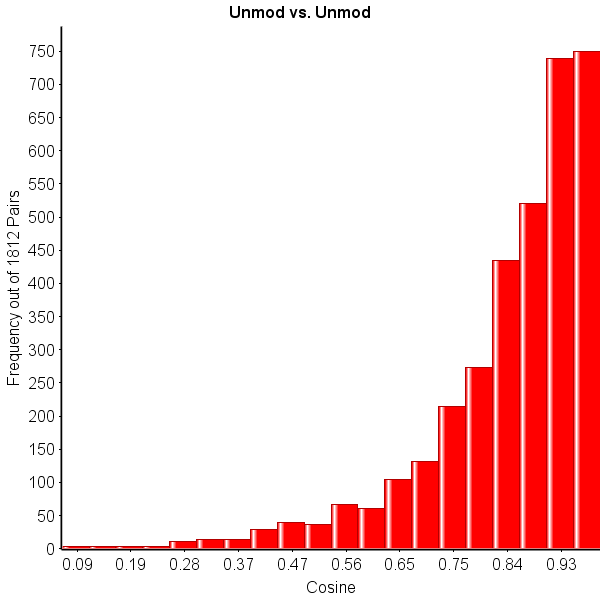
\includegraphics[width=2in,height=2in]{fig/lens/cosine_unmod_vs_unmod.png}
b)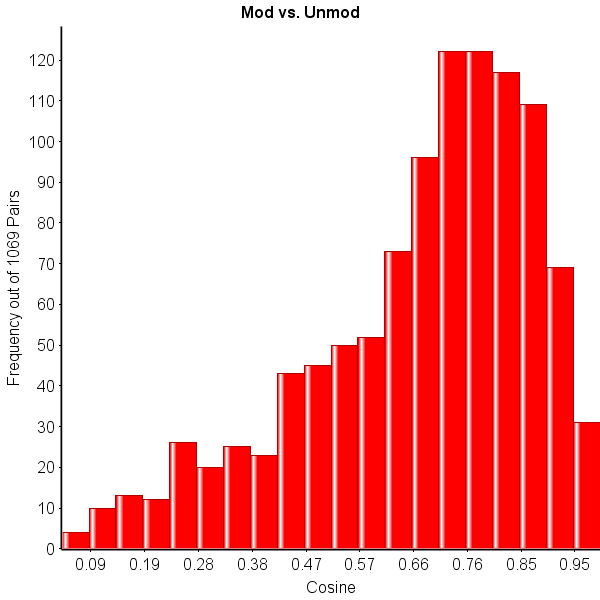
\includegraphics[width=2in,height=2in]{fig/lens/cosine_mod_vs_unmod.png}
c)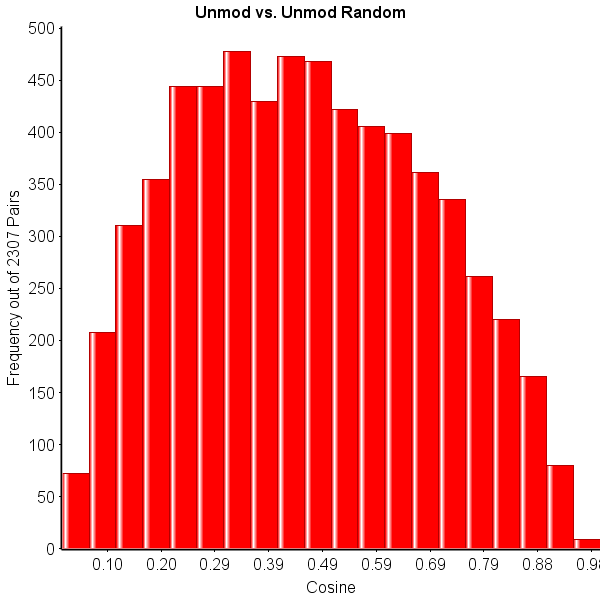
\includegraphics[width=2in,height=2in]{fig/lens/cosine_random_unmod.png}\\
d)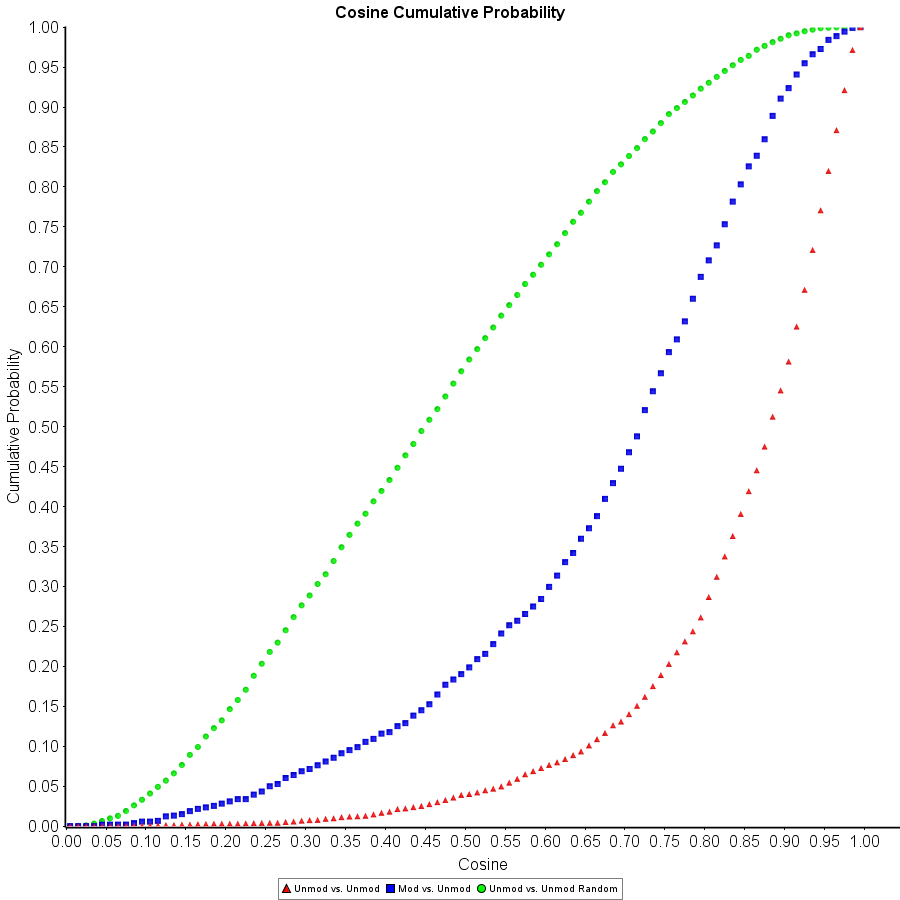
\includegraphics[width=3in,height=3in]{fig/lens/cosine_cumulative_probablility.png}
\caption{Charge 2 Lens Dataset: Distribution of cosine score of (a) top scoring unmodified spectrum of a peptide vs. top five matching spectra with the same peptide annotation. (b) top scoring unmodified spectrum of a peptide vs. top five matching spectra with the same peptide sequence, but with modifications. (c) unmodified peptides of differing sequences of the same length and within 20 $m/z$ (d) Cumulative probability distribution of cosine scores of charge 2 spectra of random peptides with similar mass and same length, the same unmodified peptide, unmodified and modified versions of the same peptide.}
\label{fig:CosineScoreDist}
\end{figure}

\begin{figure}[htbp]
\centering % trim=l b r t
a)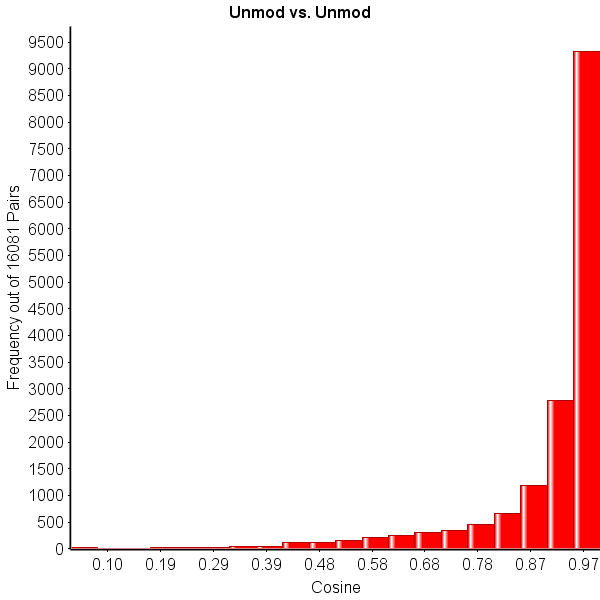
\includegraphics[width=2in,height=2in]{fig/phospho/cosine_unmod_vs_unmod.png}
b)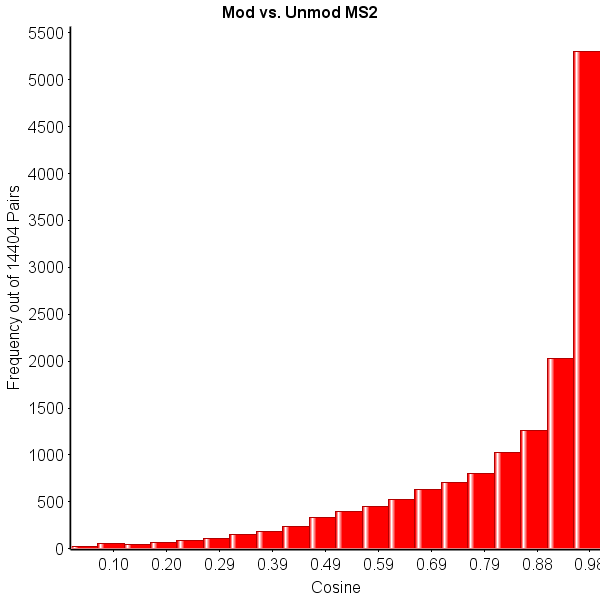
\includegraphics[width=2in,height=2in]{fig/phospho/cosine_mod_vs_unmod_ms2.png}
c)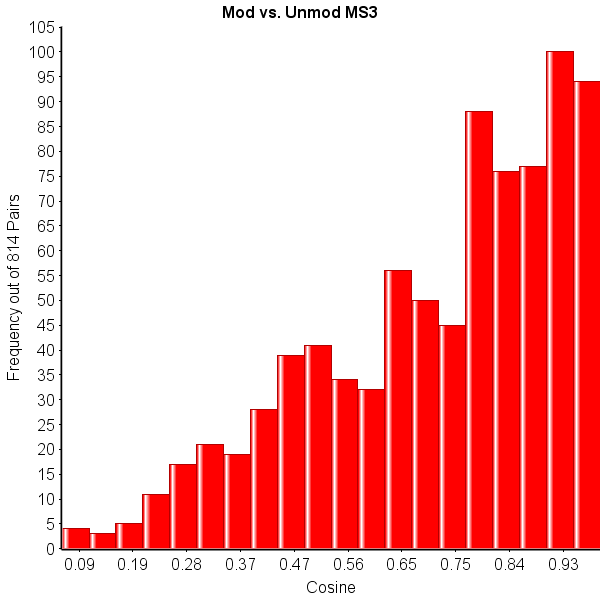
\includegraphics[width=2in,height=2in]{fig/phospho/cosine_mod_vs_unmod_ms3.png}
d)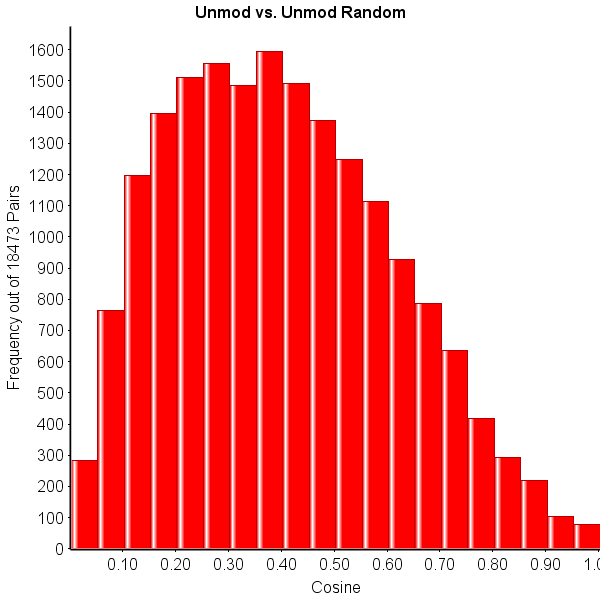
\includegraphics[width=2in,height=2in]{fig/phospho/cosine_unmod_vs_unmod_random.png} \\
e)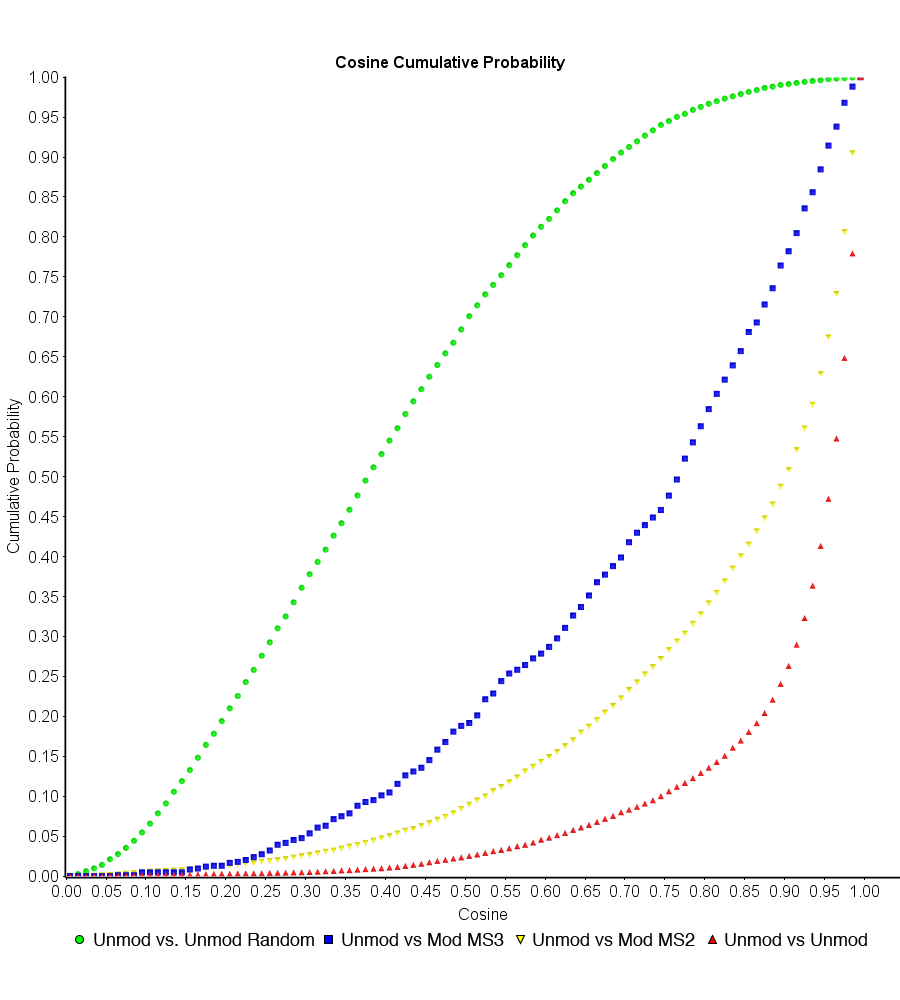
\includegraphics[width=3in,height=3in]{fig/phospho/cumulative_probability.png}
\caption{Charge 2 Yeast dataset: Distribution of cosine score of (a)top scoring unmodified spectrum of a peptide vs. top five matching spectra with the same peptide annotation. (b) top scoring unmodified spectrum of a peptide vs. top five matching spectra with the same peptide sequence, but with modifications. (c)unmodified peptides of differing sequences of the same length and within 20 $m/z$  (d) Cumulative probability distribution of cosine scores of spectra of random peptides with similar mass, the same unmodified peptide, unmodified and dehydrated versions of the same peptide for MS2 and MS3.}
\label{fig:Yeast_CosineScoreDist}
\end{figure}

For our CID spectra for the yeast phospho datasets, the similarity of 
the predicted unmodified spectra to the real unmodified and modified spectra were very high. For MS2 modified spectra, $85.00\%$ 
of the predicted MassAnalyzer unmodified spectra still had a cosine score of greater than $.4$. For MS3 modified spectra, $88.68\%$ were above $.4$. 
While this isn't as high as the values for unmodified experimental spectra which were $94.98\%$ for modified MS2 and $89.5\%$ for modified MS3 respectively,
in cases where the experimental unmodified spectra isn't available, we can see that 
MassAnalyzer still produces reasonable spectra. Figure~\ref{fig:CosineMassAnalyzer}

\begin{figure}[htbp]
\centering
a)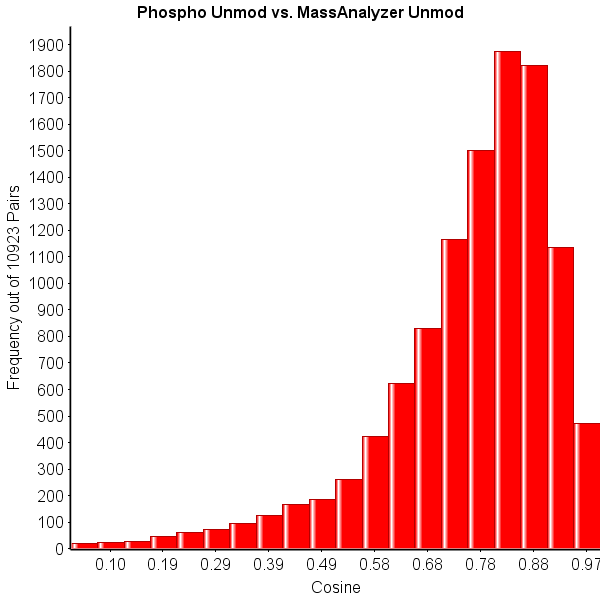
\includegraphics[width=2in,height=2in]{fig/phospho/cosine_unmod_vs_massanalyzer.png}
b)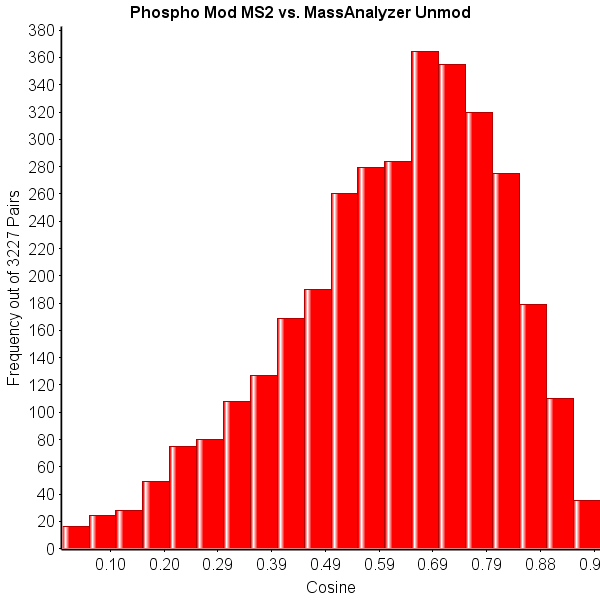
\includegraphics[width=2in,height=2in]{fig/phospho/cosine_mod_ms2_vs_massanalyzer.png}
c)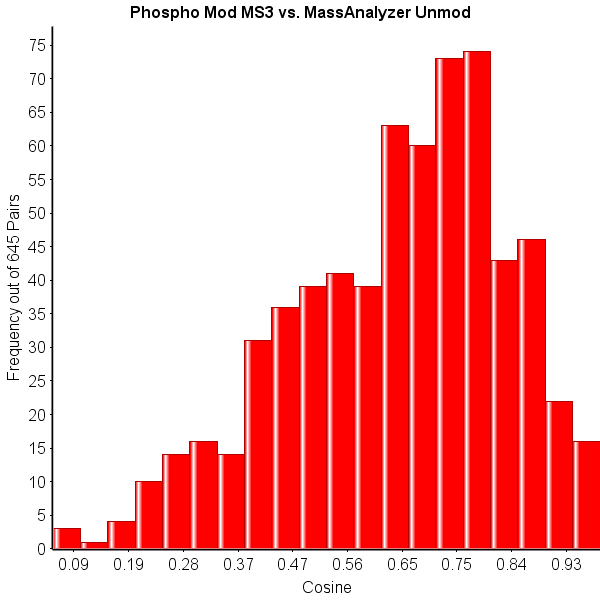
\includegraphics[width=2in,height=2in]{fig/phospho/cosine_mod_ms3_vs_massanalyzer.png}
\caption{Charge 2 Yeast dataset: Distribution of cosine score of (a) unmodified MS2 spectra vs. unmodified predicted MassAnalyzer MS2 spectra 
(b) modified MS2 spectra vs unmodified predicted MassAnalyzer MS2 spectra (c) modified MS3 spectra vs. unmodified predicted MassAnalyzer spectra.}
\label{fig:CosineMassAnalyzer}
\end{figure}

For our synthetic human phosphorylated peptides, in Figure~\ref{fig:CosineSynthetic}, we can see that the similarity still 
quite high.

\begin{figure}[htbp]
\centering
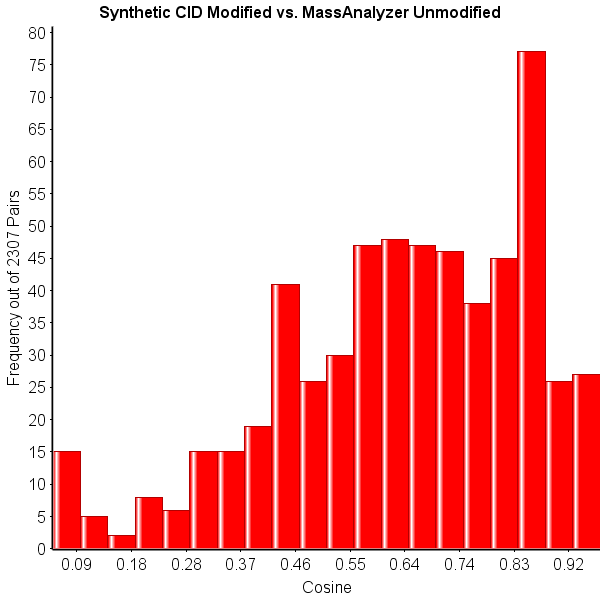
\includegraphics[width=2in,height=2in]{fig/phospho/cosine_mod_vs_massanalyzer_synthetic_cid.png}
\caption{Mascot synthetic dataset: Distribution of cosine score of MassAnalyzer CID unmodified spectral prediction vs. modified synthetic spectrum for CID spectra}
\label{fig:CosineSynthetic}
\end{figure}

Since it is possible to estimate peak intensities for modified spectra from unmodified spectra, it is possible to calculate theoretical peak intensities for modified variants of a peptide using the unmodified spectrum. Assuming we are given a modified spectrum $S'$ from modified peptide $P'$ whose unmodified version is $P$, we choose from a set of spectra $S_1 \cdots S_n$ all from peptide $P$. We then choose the spectrum $S_{i}$ with the highest cosine similarity to $S'$. The $S$ is normalized to a total intensity of 1000000. We then take $Intensities(S,P)$. If a peak from $S$ is annotated with a single fragment ion, we assign the peak intensity as the expected intensity of that fragment ion. If a peak is annotated by 
multiple fragment ions, it is possible to choose from several strategies such as splitting the peak intensity among the ions according to their estimated ion probabilities or PRM scores, etc. Our results did not differ much with different strategies, so we adopted a simpler strategy. If a peak is annotated by multiple fragment ions, we assign the whole intensity to the ion
with largest ion probability. For every other fragment ion not detected in the unmodified spectrum, we assign a detectability of $\epsilon > 0$. In our tests we used $\epsilon=1$.

\subsection{Quantification of Modification Variants via Linear Programming}\label{sec:quantificationSupplemental}

The mixture spectrum of modification variants is the superposition of individual modified spectra from all of the modification variants. Therefore, a peak intensity does not necessarily correspond to a fragment ion from a single parent modification variant. Most often, multiple fragment ions from one or more variants have the same m/z value and contribute to the same peak. In the case of a singly modified peptide, for example, only y1 and b1 would be contributing to a single variant (the first and last modification positions). All other b and y ions would be shared between multiple variants.

For instance, in the simple example shown in Figure~\ref{fig:3by5example}, in the presence of all variants, the intensity of a b3 modified peak will be contributed to by three different variants. Note that since we have an equal mixture of all four variants, the intensity in the modified spectrum of b3 is $1:3$ between the unmodified and modified ion. It is crucial to see the mapping between the peaks and the theoretical fragment ions as well as the mapping between variants and the fragment ions. Each observed intensity value in the mixture spectrum at a theoretical m/z value gives information about the total abundance of the fragment ions from variants contributing to that peak.

\begin{figure}[htbp!]
\centering
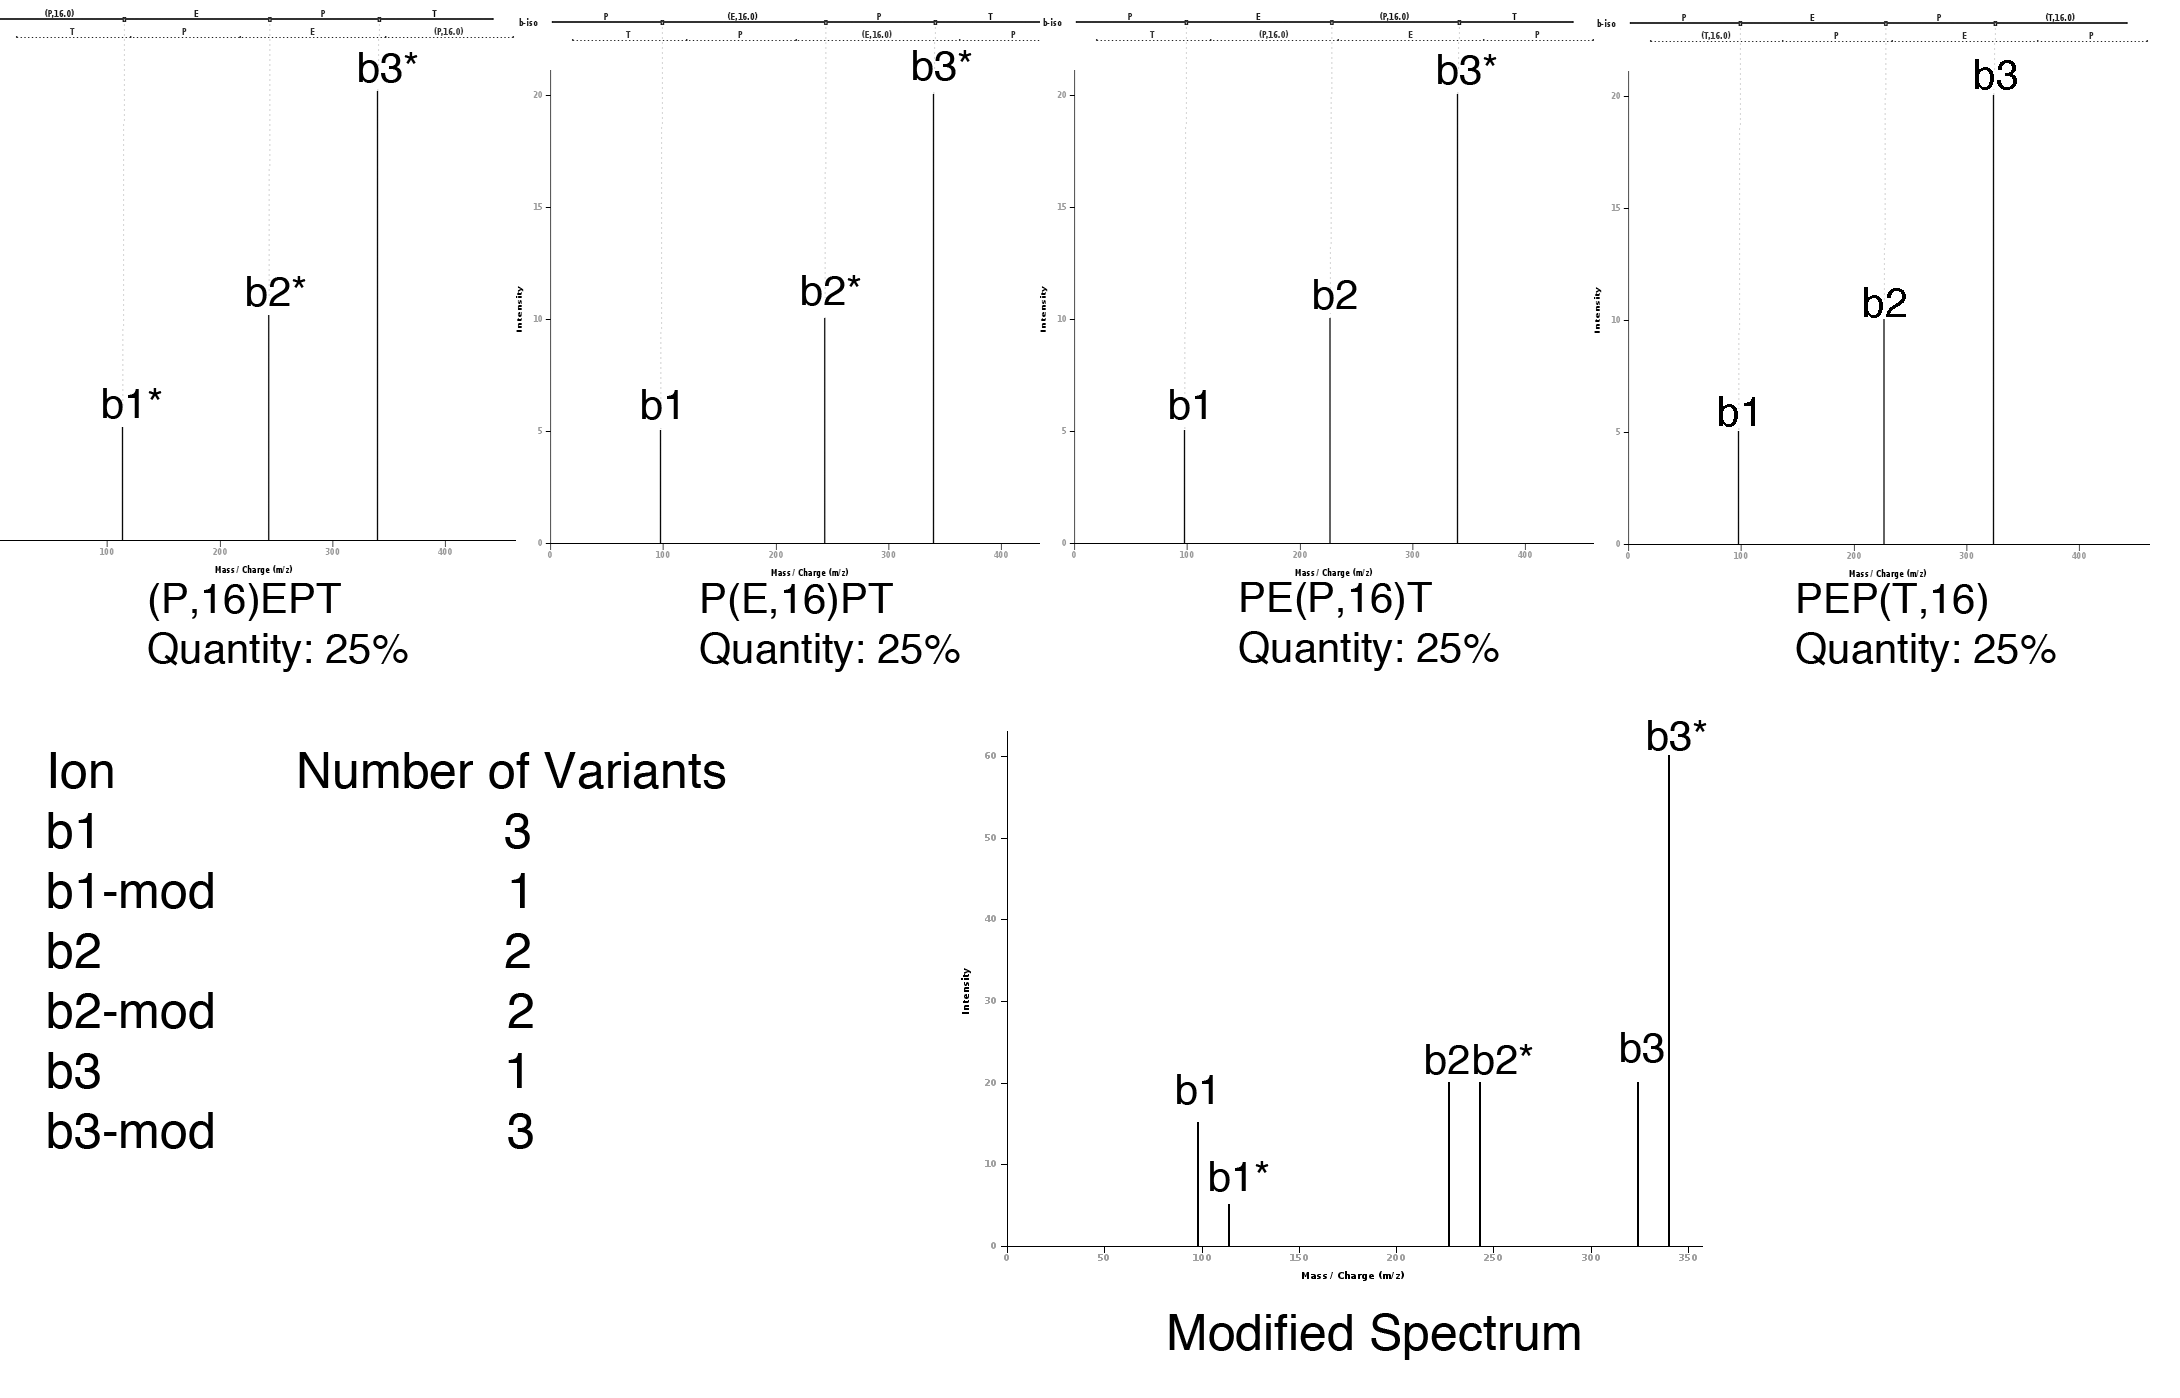
\includegraphics[]{PEPT_all.png}
\caption{Given a set of variants, (P,16)EPT, P(E,16)PT, PE(P,16)T and PEP(T,16), we assume that the spectra of all three modified peptides will be similar to the unmodified spectrum PEPT (not shown). If we have equal quantities of all possible variants, then the intensity of each peak can be contributed to by more than one variant. In this case, since b1 unmodified and b3 modified are only contributed to by one variant, the modified and unmodified peaks have a ratio of 3:1 and 1:3 respectively. The b2 peak has two variants contributing to both the unmodified and modified versions, so it has a ratio of 2:2.}
\label{fig:3by5example}
\end{figure}